\renewcommand{\thesection}{A.\arabic{section}}
\setcounter{section}{0}
\setcounter{equation}{0}
\renewcommand{\theequation}{A.\arabic{equation}}
\renewcommand{\theHequation}{A.\arabic{equation}}

\section{Derivation of the elasticity of taxable income}

This appendix derives the elasticity used in Section 1 from the taxpayer's optimality condition.

\subsection{Preferences and the intensive-margin choice.} 
Consider a taxpayer indexed by unobserved earning ability $n > 0$ (which captures productivity or ease of generating income) who derives utility from disposable consumption $c$ and suffers disutility from producing and reporting taxable income $z$ (encompassing labor effort, tax avoidance, and reporting costs). Preferences take the standard quasilinear, isoelastic form:
\begin{equation}
u(c,z) = c - \frac{n^{-1/\epsilon}}{1+1/\epsilon}\,z^{1+1/\epsilon},
\label{eq:app_utility}
\end{equation}
where $\epsilon > 0$ governs the curvature of the disutility of income generation. Because the second term is strictly convex in $z$ and scaled by $n^{-1/\epsilon}$, higher-ability taxpayers face a lower marginal cost of generating any given level of taxable income. Figure~\ref{fig:disutility_curvature} illustrates how $\epsilon$ shapes both total disutility (left panel) and the marginal cost of generating income (right panel) around the benchmark ability level $z = n$. When $\epsilon$ is small (e.g., $\epsilon = 0.2$), the disutility function is sharply curved and marginal cost rises steeply above $n$, implying that taxpayers adjust their reported income very little in response to changes in the net-of-tax rate. Conversely, as $\epsilon$ increases (e.g., $\epsilon = 2.0$), the disutility schedule becomes flatter and marginal cost varies slowly with $z$, leading to larger intensive-margin adjustments when tax incentives change.

\begin{figure}[htbp]
    \centering
    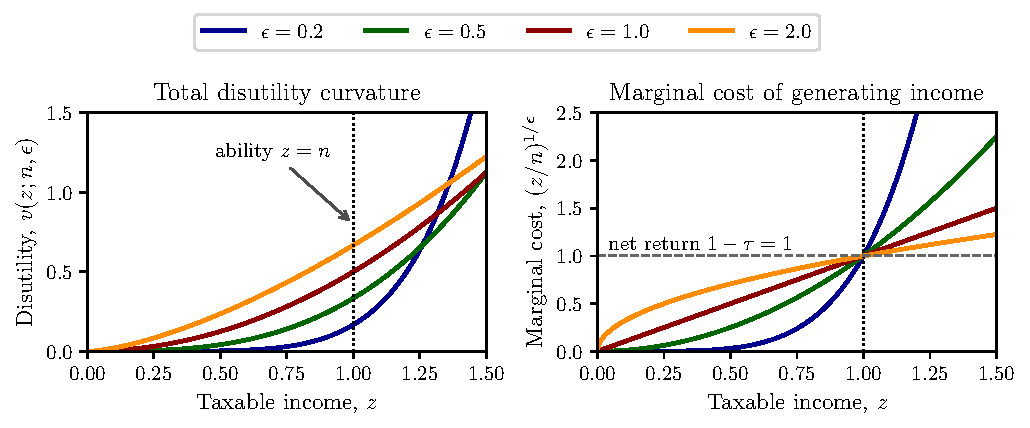
\includegraphics[width=0.95\textwidth]{disutility_curvature.pdf}
    \caption{\textbf{Curvature of isoelastic disutility and marginal cost across ETI values.} The left panel plots total disutility $v(z; n, \epsilon) = \frac{n}{1+1/\epsilon}(z/n)^{1+1/\epsilon}$ and the right panel plots the corresponding marginal cost $v_z(z; n, \epsilon) = (z/n)^{1/\epsilon}$ for normalized ability $n = 1$ across different values of the elasticity of taxable income $\epsilon$. Lower values of $\epsilon$ generate steeper curvature around $z = n$, damping behavioral responses to tax rate changes.}
    \label{fig:disutility_curvature}
\end{figure}

The taxpayer maximizes \eqref{eq:app_utility} subject to a linear budget constraint:
\begin{equation}
c = (1-\tau)z + R,
\label{eq:app_budget}
\end{equation}
where $\tau \in [0,1)$ is the constant marginal tax rate, $(1-\tau)$ is the net-of-tax rate (the marginal return to earning and reporting an extra unit of income), and $R$ denotes unearned or virtual income (such as non-labor income or lump-sum transfers).

Substituting the budget constraint into utility and taking the first-order condition with respect to $z$ yields:
\begin{equation}
1-\tau = n^{-1/\epsilon}z^{1/\epsilon}.
\label{eq:app_foc}
\end{equation}
Economically, the taxpayer expands taxable income until the marginal private benefit of an additional peso of declared income---the net-of-tax rate $(1-\tau)$---equals the marginal disutility cost of generating it, $(z/n)^{1/\epsilon}$. Solving \eqref{eq:app_foc} for $z$ characterizes optimal declared income:
\begin{equation}
z(n;\tau) = n\,(1-\tau)^{\epsilon}.
\label{eq:app_choice}
\end{equation}
This supply function separates baseline potential from tax incentives: in a tax-free benchmark ($\tau = 0$), a taxpayer simply declares their ability ($z = n$), whereas positive marginal taxes scale down reported income proportionally across all ability types.

Finally, the elasticity of taxable income (ETI) is defined as the percentage change in declared income induced by a one-percent change in the net-of-tax rate, holding ability fixed:
\begin{equation}
\epsilon \equiv \frac{\partial \ln z(n;\tau)}{\partial \ln (1-\tau)}.
\label{eq:app_eti}
\end{equation}
Taking logs of \eqref{eq:app_choice} gives $\ln z(n;\tau) = \ln n + \epsilon \ln(1-\tau)$, so differentiating immediately confirms $\partial \ln z / \partial \ln(1-\tau) = \epsilon$. This isoelastic specification is analytically convenient because the ETI is constant across all income levels and directly equals the structural preference parameter $\epsilon$. Moreover, because utility is linear in consumption $c$, optimal income \eqref{eq:app_choice} is independent of virtual income $R$: there are no income effects, ensuring that \eqref{eq:app_eti} represents both the compensated and uncompensated elasticity.


\subsection{The kink and the marginal buncher.}
While a linear tax schedule induces a smooth mapping from unobserved ability $n$ to declared income $z(n;\tau) = n(1-\tau)^{\epsilon}$, actual income tax systems are piecewise linear, featuring discrete increases in marginal tax rates at bracket cutoffs. To see how such nonlinearities map behavioral elasticities into observable clustering, suppose the marginal tax rate jumps from $\tau_0$ below an exemption or bracket threshold $z^*$ to $\tau_1 > \tau_0$ above it, generating the piecewise-linear budget set\footnote{We normalize virtual income to $R = 0$ without loss of generality; because preferences \eqref{eq:app_utility} are quasilinear in consumption, any additive intercept shifts consumption vertically without affecting optimal taxable income $z(n)$ or the bunching thresholds.}
\begin{equation}
c = \begin{cases}
(1-\tau_0)z & \text{if } z < z^{*},\\[2pt]
(1-\tau_0)z^{*} + (1-\tau_1)(z-z^{*}) & \text{if } z \ge z^{*}.
\end{cases}
\label{eq:app_kink}
\end{equation}
Because $\tau_1 > \tau_0$, the budget set is continuous at $z^*$ but exhibits a convex kink where the net-of-tax return falls discretely from $1-\tau_0$ to $1-\tau_1$ (See Figure \ref{fig:kink_notch} for a visual representation). 

Substituting \eqref{eq:app_kink} into \eqref{eq:app_utility} yields a strictly concave objective $U(z;n)$ with a corner at $z^*$, where standard differentiability fails.\marginnote{Directional marginal utility refers to the left- and right-hand derivatives of objective utility at a kink point $z^*$ ($U'_-(z^*)$ and $U'_+(z^*)$), measuring the marginal net gain of approaching or crossing the threshold when standard differentiability fails.} Rather than setting a single derivative to zero, optimality at the threshold requires directional marginal utility to be non-negative approaching $z^*$ from the left and non-positive departing from the right:
\begin{equation}
U_{-}'(z^*;n) = (1-\tau_0) - \left(\frac{z^*}{n}\right)^{1/\epsilon} \ge 0
\qquad\text{and}\qquad
U_{+}'(z^*;n) = (1-\tau_1) - \left(\frac{z^*}{n}\right)^{1/\epsilon} \le 0.
\label{eq:app_directional}
\end{equation}
Intuitively, a taxpayer prefers to remain at $z^*$ rather than reducing income if the lower-bracket net return $1-\tau_0$ still covers the marginal disutility of reaching $z^*$, and prefers not to expand beyond $z^*$ if the higher-bracket net return $1-\tau_1$ falls short of that marginal cost. Figure~\ref{fig:directional_utility_kink} illustrates this mechanism across three representative ability types. While every taxpayer experiences a discrete downward jump of size $\tau_1 - \tau_0$ in marginal utility at $z^*$ (right panel), only intermediate-ability types straddle zero across the discontinuity ($U'_-(z^*;n) > 0 > U'_+(z^*;n)$), locking their maximum onto a sharp corner peak at $z^*$ (left panel).

\begin{figure}[htbp]
    \centering
    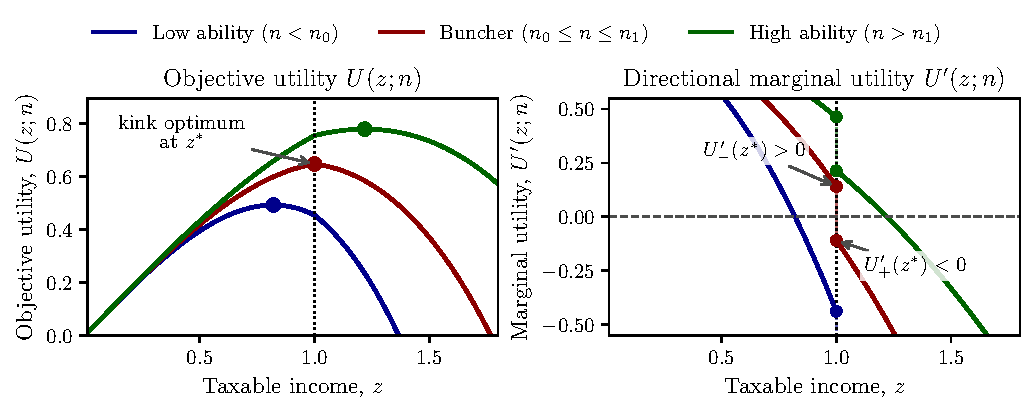
\includegraphics[width=0.95\textwidth]{directional_utility_kink.pdf}
    \caption{\textbf{Objective utility and directional marginal utility at a convex kink.} The left panel plots objective utility $U(z;n) = c(z) - v(z;n)$ and the right panel plots marginal utility $U'(z;n)$ across three ability types around the kink threshold $z^* = 1$ ($\tau_0 = 0.10$, $\tau_1 = 0.40$, $\epsilon = 0.5$). Low-ability taxpayers ($n < n_0$) reach an interior optimum strictly below $z^*$, and high-ability taxpayers ($n > n_1$) remain above $z^*$ even after the marginal rate increase. For intermediate types ($n_0 \le n \le n_1$), marginal utility jumps from positive ($U'_-(z^*) > 0$) to negative ($U'_+(z^*) < 0$) at $z^*$, producing a corner optimum at the threshold.}
    \label{fig:directional_utility_kink}
\end{figure}

Combining both conditions in \eqref{eq:app_directional} yields $1-\tau_1 \le (z^*/n)^{1/\epsilon} \le 1-\tau_0$, which is algebraically equivalent to $z_1(n) \le z^* \le z_0(n)$. Partitioning taxpayers across the full ability distribution gives the piecewise optimal income schedule:
\begin{equation}
z(n)=
\begin{cases}
z_0(n) = n(1-\tau_0)^{\epsilon} & \text{if } z_0(n) \le z^{*},\\[2pt]
z^{*} & \text{if } z_1(n) < z^{*} < z_0(n),\\[2pt]
z_1(n) = n(1-\tau_1)^{\epsilon} & \text{if } z_1(n) \ge z^{*},
\end{cases}
\label{eq:app_solution}
\end{equation}
where $z_0(n)$ and $z_1(n)$ denote unconstrained optimal choices under constant marginal rates $\tau_0$ and $\tau_1$, respectively. Low-ability taxpayers ($z_0(n) \le z^*$) remain strictly below the cutoff and are unaffected at the margin, while high-ability taxpayers ($z_1(n) \ge z^*$) locate in the interior of the upper bracket. Crucially, the intermediate group---those who would choose above $z^*$ under $\tau_0$ but prefer below $z^*$ under $\tau_1$---collapses onto the single point $z^*$, transforming a continuous interval of unobserved abilities into a discrete point mass (excess bunching) in the observed income distribution.

The upper bound of this bunching interval is pinned down by the \emph{marginal buncher}, defined as the highest-ability taxpayer $n_B$ who locates at the kink---that is, the type whose unconstrained optimum under the higher tax rate $\tau_1$ coincides exactly with the threshold, $z_1(n_B) = z^*$. Inverting $z_1(n_B) = n_B(1-\tau_1)^{\epsilon} = z^*$ recovers this taxpayer's unobserved ability:
\begin{equation}
n_B = z^{*}(1-\tau_1)^{-\epsilon}.
\label{eq:app_nb}
\end{equation}
Next, we ask what income this same marginal taxpayer would have declared in a counterfactual linear schedule where the lower rate $\tau_0$ applied throughout. Substituting \eqref{eq:app_nb} into the unconstrained supply function $z_0(n_B) = n_B(1-\tau_0)^{\epsilon}$ yields
\begin{equation}
z_0(n_B) = \left[z^{*}(1-\tau_1)^{-\epsilon}\right](1-\tau_0)^{\epsilon} = z^{*}\left(\frac{1-\tau_0}{1-\tau_1}\right)^{\epsilon}.
\label{eq:app_buncher}
\end{equation}
Thus, in the absence of the kink, all bunching taxpayers would have distributed smoothly across the counterfactual interval $(z^*, z_0(n_B)]$, whose width $\Delta z^* \equiv z_0(n_B) - z^*$ increases monotonically with the elasticity $\epsilon$.


\subsection{Excess mass}
While the optimization model characterizes bunching in terms of a latent counterfactual income band $(z^*, z_0(n_B)]$ of width $\Delta z^* \equiv z_0(n_B) - z^*$, empirical tax data only reveal the discrete number of taxpayers clustering at the threshold. Translating this observed mass back into an income distance requires knowing how densely populated the neighborhood of $z^*$ would have been in the absence of the kink.

Let $g(z)$ denote the counterfactual density of taxable income (expressed in taxpayers per peso) that would prevail under the smooth linear schedule with rate $\tau_0$. Because all taxpayers who relocate to $z^*$ are drawn from the counterfactual interval $(z^*, z_0(n_B)]$, the total excess mass $B$ of bunching taxpayers at the threshold is given by integrating $g(z)$ over this range:
\begin{equation}
B = \int_{z^{*}}^{z_0(n_B)} g(v)\,dv \;\approx\; g(z^{*})\,\bigl[z_0(n_B)-z^{*}\bigr]
\;\equiv\; g(z^{*})\,\Delta z^{*},
\label{eq:app_B}
\end{equation}
where the approximation assumes that the counterfactual density is locally uniform across the bunching band, $g(v) \approx g(z^*)$ for $v \in (z^*, z_0(n_B)]$. Figure~\ref{fig:excess_mass_identification} illustrates this geometric equivalence: the excess pile-up $B$ observed above the smooth counterfactual density at $z^*$ corresponds to the area under $g(z)$ over $(z^*, z^* + \Delta z^*]$, which is approximated by a rectangle of height $g(z^*)$ and base $\Delta z^*$. Intuitively, for a given observed pile-up $B$, a lower counterfactual density $g(z^*)$ implies that bunchers had to travel from further up the income distribution (a larger $\Delta z^*$). Normalizing the excess mass by the counterfactual height at the threshold defines the normalized bunching statistic:
\begin{equation}
b \equiv \frac{B}{g(z^{*})} \approx \Delta z^{*}.
\label{eq:app_b_norm}
\end{equation}
Because $B$ is a count of taxpayers and $g(z^*)$ is measured in taxpayers per peso, $b$ is expressed directly in monetary units of taxable income and provides a direct empirical counterpart to the unobserved counterfactual response $\Delta z^*$.

\begin{figure}[htbp]
    \centering
    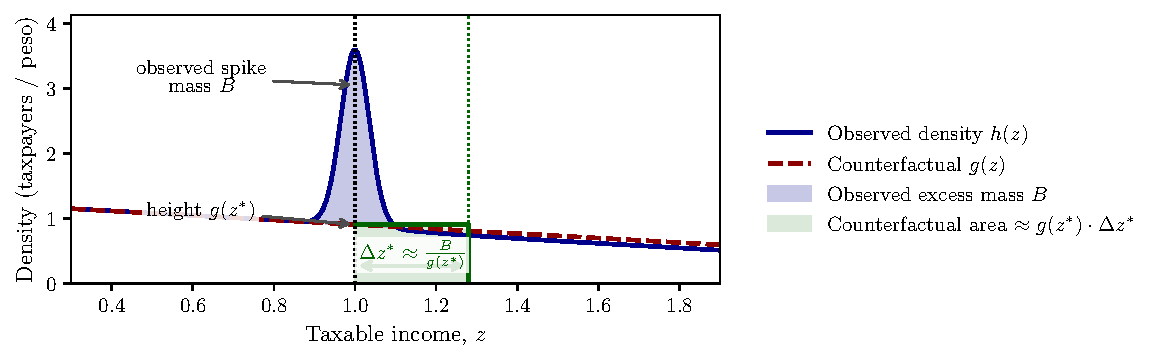
\includegraphics[width=0.99\textwidth]{excess_mass_identification.pdf}
    \caption{\textbf{Identification of the counterfactual response width $\Delta z^*$ from observed excess mass $B$.} The figure compares the observed taxable income density $h(z)$ (solid blue) with the smooth counterfactual density $g(z)$ interpolated from unaffected neighbors (dashed red) around the kink threshold $z^*$. The excess mass $B$ accumulated above $g(z)$ at $z^*$ equals the missing counterfactual mass over $(z^*, z^* + \Delta z^*]$. Under local uniformity, this area is approximated by the green rectangle $g(z^*) \cdot \Delta z^*$, allowing $\Delta z^*$ to be recovered as $B / g(z^*)$.}
    \label{fig:excess_mass_identification}
\end{figure}

\subsection{From excess mass to the elasticity}
Having linked the empirical bunching statistic $b$ to the counterfactual income width $\Delta z^*$, we can invert the structural relationship derived in \eqref{eq:app_buncher} to recover the elasticity of taxable income. Substituting $z_0(n_B) = z^*\bigl[(1-\tau_0)/(1-\tau_1)\bigr]^{\epsilon}$ into the definition $\Delta z^* \equiv z_0(n_B) - z^*$ and dividing by $z^*$ expresses the percentage income response of the marginal buncher as a function of the tax jump:
\begin{equation}
\frac{\Delta z^{*}}{z^{*}} = \left(\frac{1-\tau_0}{1-\tau_1}\right)^{\epsilon} - 1
\quad\Longleftrightarrow\quad
\ln\left(1+\frac{\Delta z^{*}}{z^{*}}\right) = \epsilon\,\ln\left(\frac{1-\tau_0}{1-\tau_1}\right).
\label{eq:app_log}
\end{equation}
Replacing the latent width $\Delta z^*$ with its empirical proxy $b$ from \eqref{eq:app_b_norm} yields the exact closed-form parametric estimator for $\epsilon$ under locally uniform density. Moreover, when the kink is small so that $\Delta z^*/z^*$ is close to zero, applying the first-order Taylor expansion $\ln(1+x) = x + O(x^2)$ produces the standard Saez-style linear approximation:
\begin{equation}
\epsilon = \frac{\ln\left(1+\Delta z^{*}/z^{*}\right)}{\ln\left(\frac{1-\tau_0}{1-\tau_1}\right)}
\;\approx\;
\frac{\Delta z^{*}}{z^{*}\ln\left(\frac{1-\tau_0}{1-\tau_1}\right)}
\;\approx\;
\frac{b}{z^{*}\ln\left(\frac{1-\tau_0}{1-\tau_1}\right)}.
\label{eq:app_final}
\end{equation}
Equation~\eqref{eq:app_final} completes the mapping from theoretical preferences to empirical estimation: the numerator $b/z^*$ captures the normalized behavioral response inferred from the excess mass at the threshold, while the denominator $\ln\bigl((1-\tau_0)/(1-\tau_1)\bigr) \approx (\tau_1 - \tau_0)/(1-\tau_0)$ measures the percentage reduction in the net-of-tax rate induced by the kink.


\section{Multi-Year Pooled Bunching Extensions (2005--2023)}
\label{app:pooled_bunching}

To examine whether the cross-sectional estimates for 2023 are affected by single-year sampling noise or year-specific administrative reporting patterns, this appendix extends the baseline polynomial bunching estimator (including iterative right-tail reweighting) by pooling all 19 available annual distributions in the SII administrative records (2005--2023).

\subsection{Pooling across years via statutory normalization}

Because the Chilean personal income tax exemption threshold $K_t$ is defined in nominal pesos (indexed to the \textit{Unidad Tributaria Anual}, UTA) and updated every year, annual taxable incomes cannot be stacked directly in levels: a pile-up in 2005 and a pile-up in 2023 fall in different nominal brackets, and raw aggregation would smooth away the behavioral spike. To align the statutory kink across time, each year's bin edges are rescaled by that year's statutory annual exemption cutoff $K_t$,
\begin{equation}
\tilde{z}_{j,t} = \frac{z_{j,t}}{K_t},
\end{equation}
so that the statutory kink maps to $\tilde{z}^* = 1$ in every year $t \in \{2005, \dots, 2023\}$. Counts are then aggregated onto a common grid of width $\Delta \tilde{z} = 0.01$ threshold units.

Maintaining the fourth-degree polynomial specification with iterative right-tail reweighting and the 2023 baseline window and exclusion boundaries rescaled in threshold units---namely a fitting window of $[0.625,\, 1.923]$ and an excluded bunching region of $[0.817,\, 1.009)$. The pooled excess mass is $\hat{B} = 206{,}823$ taxpayers ($\hat{b} = 0.0137$ threshold units) and the resulting elasticity is $\hat{\epsilon} = 0.3356$ (Figure~\ref{fig:p1_pooled}). While pooling reduces finite-sample variance and makes the local discontinuity visually sharper, it does not eliminate sensitivity to the polynomial fitting window, as the counterfactual remains a fourth-degree extrapolation over a truncated support. Moreover, statutory normalization introduces an alignment caveat: because the empirical pile-up often peaks slightly below the legal cutoff $K_t$ due to optimization frictions and income lumpiness, statutory rescaling places yearly modes in slightly different normalized bins.

\begin{figure}[htbp]
\centering
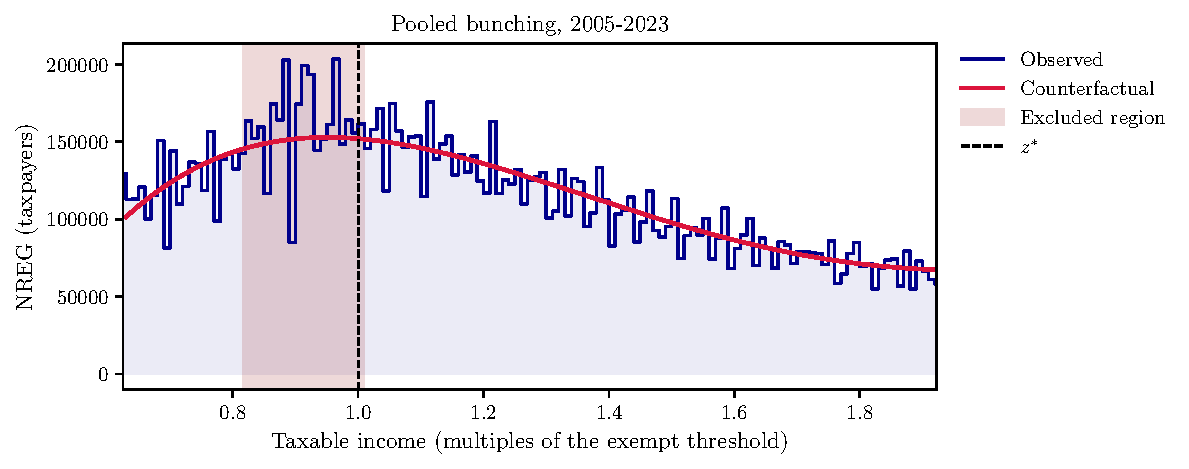
\includegraphics[width=\textwidth]{p1/p1_pooled_bunching.pdf}
\caption{Bunching pooled over 2005--2023 under statutory threshold normalization. Income is expressed in units of each year's statutory exemption cutoff $K_t$, mapping the legal kink to $\tilde{z}^* = 1$ in every year. Bars show pooled taxpayer counts, the red curve shows the fitted counterfactual, and the shaded band indicates the excluded region.}
\label{fig:p1_pooled}
\end{figure}

\subsection{Aligning on the empirical pile-up}

Statutory normalization assumes that dividing by $K_t$ places every year's empirical bunching spike in the exact same bin. Table~\ref{tab:app_peak_ratio} and Figure~\ref{fig:app_peak_ratio_trend} report the year-by-year diagnostic from 2005 to 2023, comparing each year's statutory exemption threshold $K_t$ with the empirical local mode $m_t$ within the $[0.75\,K_t,\, 1.05\,K_t]$ neighborhood. Across the 19 years, the ratio $m_t / K_t$ averages $0.9486$ with a standard deviation of $0.0305$ (roughly $3.1$ grid bins of $0.01$ units), ranging from $0.868$ in 2022 to $1.009$ in 2009. Because this gap varies across years and exhibits a downward drift in recent years, stacking by $K_t$ disperses the annual spikes across adjacent bins and attenuates the visible peak.

\begin{table}[htbp]
\centering
\caption{Annual statutory PIT exemption threshold ($K_t$), empirical local mode ($m_t$), and peak-to-threshold ratio, 2005--2023.}
\label{tab:app_peak_ratio}
\small
\begin{adjustbox}{max width=\textwidth}
\begin{tabular}{cccc}
\toprule
Year & Statutory threshold $K_t$ (M CLP) & Empirical mode $m_t$ (M CLP) & Ratio ($m_t / K_t$) \\
\midrule
2005 & 5.0285 & 4.8 & 0.9546 \\
2006 & 5.1565 & 5.0 & 0.9697 \\
2007 & 5.5471 & 5.1 & 0.9194 \\
2008 & 6.0249 & 5.5 & 0.9129 \\
2009 & 5.9489 & 6.0 & 1.0086 \\
2010 & 6.0783 & 5.9 & 0.9707 \\
2011 & 6.3047 & 6.0 & 0.9517 \\
2012 & 6.4746 & 6.3 & 0.9730 \\
2013 & 6.6030 & 6.4 & 0.9693 \\
2014 & 6.9751 & 6.5 & 0.9319 \\
2015 & 7.2723 & 6.9 & 0.9488 \\
2016 & 7.4777 & 7.2 & 0.9629 \\
2017 & 7.6108 & 7.4 & 0.9723 \\
2018 & 7.8331 & 7.4 & 0.9447 \\
2019 & 8.0468 & 7.7 & 0.9569 \\
2020 & 8.2730 & 7.9 & 0.9549 \\
2021 & 8.7755 & 8.0 & 0.9116 \\
2022 & 9.9042 & 8.6 & 0.8683 \\
2023 & 10.4029 & 9.8 & 0.9420 \\
\midrule
Mean (SD) & --- & --- & 0.9486 (0.0305) \\
\bottomrule
\end{tabular}
\end{adjustbox}
\vspace{0.4em}
\begin{minipage}{0.88\textwidth}
\footnotesize \textit{Notes:} The empirical local mode $m_t$ is defined as the lower edge of the \$100,000 CLP bin with the highest taxpayer count inside $[0.75\,K_t,\, 1.05\,K_t]$.
\end{minipage}
\end{table}

\begin{figure}[htbp]
\centering
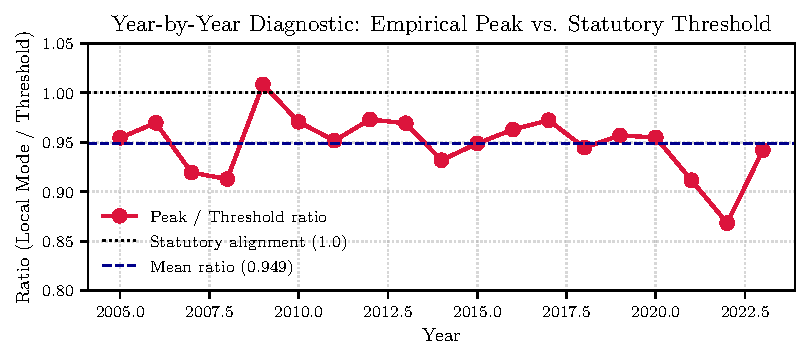
\includegraphics[width=0.9\textwidth]{p1/p1_peak_ratio_trend.pdf}
\caption{Evolution of the empirical peak to statutory threshold ratio ($m_t / K_t$), 2005--2023. The dotted line marks perfect statutory alignment ($1.0$), and the dashed line indicates the 19-year average ($0.9486$).}
\label{fig:app_peak_ratio_trend}
\end{figure}

To separate genuine behavioral bunching from cross-year misalignment, we re-pool the 2005--2023 series by normalizing each year's income by its own empirical local mode $m_t$ rather than $K_t$, placing the empirical pile-up at $\tilde{z} = 1$ by construction while keeping the estimation window and excluded region unchanged in normalized units. Under empirical-mode alignment, the pooled excess mass declines from $206{,}823$ to $166{,}065$ taxpayers and the estimated elasticity falls from $0.3356$ to $0.2899$, while the ratio of observed to counterfactual counts in the peak bin rises sharply from $1.063$ to $1.534$ (Figure~\ref{fig:p1_pooled_aligned}). This confirms that the higher statutory-pooled figure ($0.3356$) was partly inflated by cross-year peak dispersion, whereas the aligned multi-year estimate ($0.2899$) lies remarkably close to the single-year 2023 benchmark ($\hat{\epsilon}_E = 0.2799$, \parencite{gutierrezNoExemption}).

\begin{figure}[htbp]
\centering
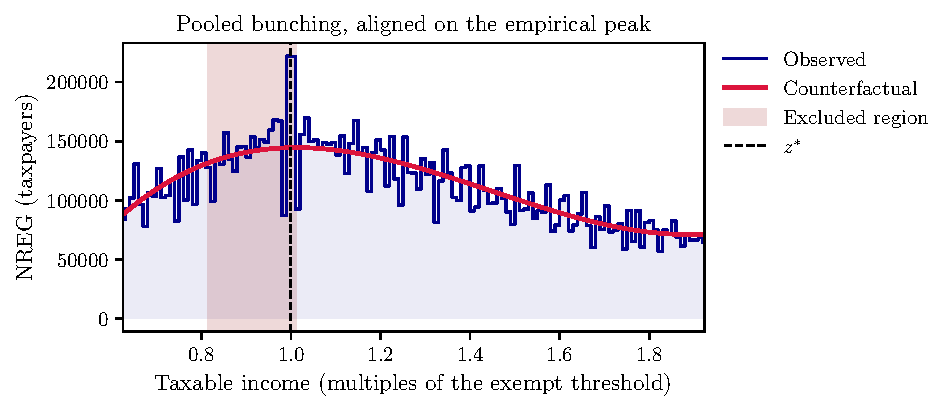
\includegraphics[width=\textwidth]{p1/p1_pooled_aligned.pdf}
\caption{Pooling aligned on the empirical pile-up, 2005--2023. Each year's income is divided by the local mode $m_t$ of its distribution around the statutory cutoff, aligning the behavioral peak at $\tilde{z} = 1$ across all years. Bars show pooled taxpayer counts, the red curve shows the fitted counterfactual, and the shaded band indicates the excluded region.}
\label{fig:p1_pooled_aligned}
\end{figure}